\chapter{Tiến hóa đa nhiệm trong huấn luyện mạng neural}
\label{mfea2}
% \section{Tiến hóa đa nhiệm dưới góc độ xác suất}
% \subsection{Mô hình hỗn hợp trong môi trường đa nhiệm}
Trong thống kê mô hình hỗn hợp (thuật ngữ gốc: \emph{mixture models}) là mô hình xác suất đại diện cho sự hiện diện của các quần thể con trong tổng thể \cite{rasmussen2000infinite}. Nói cách khác mô hình hỗn hợp là một hỗn hợp các phân phối xác suất đại diện cho các tập hợp con tạo thành quần thể.
\\[0.5cm]
\begin{figure}[h!]
    \centering
        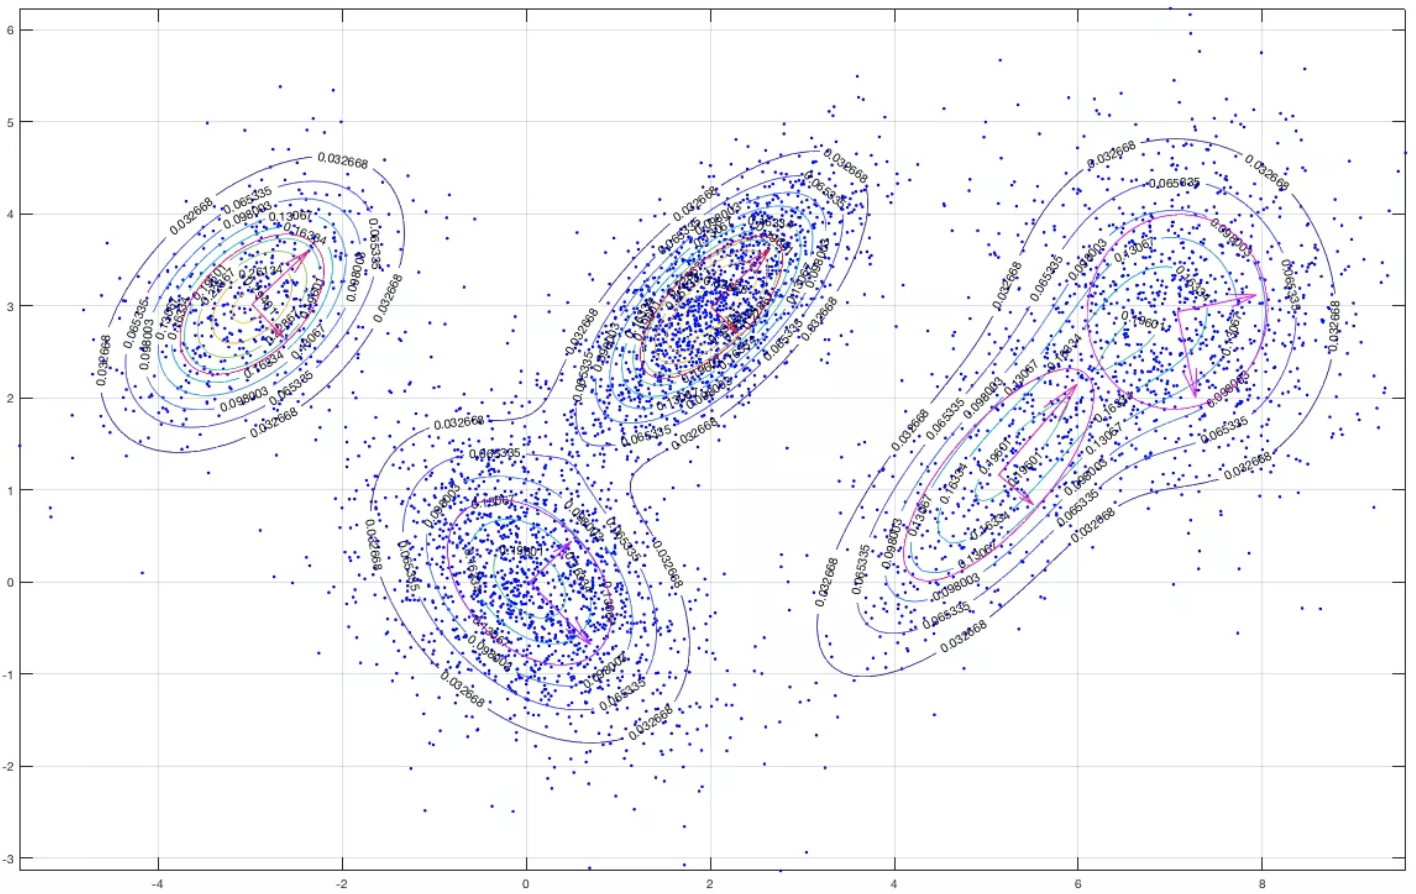
\includegraphics[width=9cm]{mixture-model.png}
    \caption{Ví dụ về mô hình hỗn hợp trong quần thể}
    \label{fig:mixture-model}
\end{figure}

Không làm mất tính tổng quát, ta coi $P^k$ là tập hợp các quần thể con liên kết với tác vụ thứ $k$ trong tập các tác vụ $k \in \{1,2,...K\}$. Hàm mục tiêu là $f_k$ và $f_k^* = f_k(x^*)$ là cực đại toàn cục tại tác vụ thứ $k$. Trong tiến hóa đa nhiệm, mỗi tác vụ các tác vụ tại một thế hệ thứ $t > 0$ có tập các quần thể con tương ứng với phân xác suất là $p^1(x,t), p^2(x,t),...., p^k(x,t)$. Sự tương tác giữa các tác vụ, quần thể con cái được sinh ra tại thế hệ thứ $t$ và bởi tác vụ thứ $k$ được biểu diễn dưới dạng một mô hình hỗn hợp như sau:
\begin{equation}
    q^k(x,t) = \alpha_k \cdot p^k(x,t) + \sum_{j \neq k} \alpha_j \cdot p^j(x,t)
    \label{equa:mixture_distribution}
\end{equation}
Ở đây phân phối $q^k(x,t)$ là một hỗn hợp $K$ phân phối với hệ số hỗn hợp là $\alpha^{'}s$. Có $\alpha_k + \sum_{j \neq k} \alpha_j = 1$ và $\alpha^{'}s >= 0$. 

Có thể thấy việc chia sẻ tri thức trong môi trường đa nhiệm là hệ quả của quá trình lấy mẫu các giải pháp phù hợp từ những phân phối hỗn hợp trong công thức \ref{equa:mixture_distribution}. Tuy nhiên trong trường hợp thiếu đi những tri thức tiên nghiệm về mối quan hệ giữa các tác vụ, việc chia sẻ tri thức có nguy cơ cao không những tri thức được chia sẻ không giúp các tác vụ tối ưu hóa nhanh hơn mà còn khiến nó bị giảm tốc độ. Hay nói cách khác là chia sẻ âm (thuật ngữ gốc: \emph{negative transfer}). Vậy vấn đề cần đặt ra là làm thế nào để xác định khi nào cần chia sẻ tri thức, khi nào không và mức độ chia sẻ là bao nhiêu. Điều này được thể hiện ở hệ số hỗn hợp $\alpha^{'}s$, giá trị $\alpha^{'}s$, và các hệ số này cần được học và tối ưu tại mỗi thế hệ sao cho phù hợp nhất với mối quan hệ giữa các tác vụ tại thời điểm đang xét.

Vậy thuật toán MFEA-I đã mô tả ở (\ref{mfeai}) với điểm nổi bật là khả năng chia sẻ tri thức giữa các tác vụ tối ưu khác nhau có gặp vấn đề negative transfer không? Dưới đây tôi sẽ đi vào phân tích thuật toán MFEA-I dưới một góc độ khác, góc độ xác suất để để trả lời cho câu hỏi đó.

\subsection{Phân tích tiến hóa đa nhiệm dưới góc độ xác suất}
Để dễ dàng phân tích thuật toán MFEA-I dưới góc độ xác suất thì không mất tính tổng quát, đưa ra một số giả thiết sau:
\begin{itemize}
    \item Toán tử sinh sản trong thuật toán MFEA-I tuân theo quy tắc xoay quanh cha mẹ (thuật ngữ gốc: \emph{parent-centric}), có nghĩa quần thể con được sinh ra có xác suất cao nằm gần với bố mẹ. 
    % Thực tế việc giả định này nhằm đơn giản việc phân tích, thay vì \emph{parent-centric} thì toán tử sinh sản ngẫu nhiên cũng sẽ có kết quả tương tự, tôi sẽ để phần chứng minh tại phụ lục bổ sung. 
    \item Phân phối xác suất của quần thể cha mẹ tuân theo phân phối chuẩn nhiều chiều.
    % với trung vị là $m$ và hiệp phương sai là $\sum$. Điều này dẫn đến hệ quả là phân phối của tập con cái sẽ rất gần với phân phối của tập cha mẹ: $p_c(x,t) \approx p(x,t)$. 
\end{itemize}
Giống như phần mô tả \emph{mô hình hỗn hợp trong môi trường đa nhiệm} ở trên, trong MFEA-I ta có thể định nghĩa lại như sau:
\begin{itemize}
    \item Tại thế hệ thứ $t$, cả $K$ tác vụ sẽ có quần thể chung là $P_t$
    \item Tại thế hệ thứ $t$ mỗi tác vụ thứ $k$ có tập quần thể con liên kết với nó là $P_t^k$
    \item $P_t$ được biểu diễn bởi mô hình $p(x,t)$, con cái của chúng được biểu diễn bởi $p_c(x,t)$
    \item $P_t^k$ được biểu diễn bởi mô hình $p^k(x,t)$, con cái của chúng được biểu diễn bởi $p_c^k(x,t)$
\end{itemize}
Tuân theo giả thiết về toán tử parent-centric, một ước lượng toàn bộ quần thể $p_c(x,t) \approx p(x,t)$. Tuy nhiên những cá thể con cái thuộc tác vụ $k$ được sinh ra do quá trình trao đổi chéo của bố mẹ là $p_c^k(x,t)$ thì \textbf{không nhất thiết phải tuân theo nguyên tắc này}.
Ta có mô hình hỗn hợp phân phối của tập con cái tại thế hệ thứ $t$ của tác vụ $k$ được biểu diễn bởi:
\begin{equation}
    p_c^k(x,t) = [1 - \frac{0.5 \cdot (K - 1) \cdot rmp}{K} ] \cdot p^k(x,t) + \sum_{j \neq k}\frac{0.5 \cdot rmp}{K} \cdot p^j(x,t).
    \label{equa:mfea_offstring_distribution}
\end{equation}
Trong đó các hệ số $\alpha_k$ và $\alpha_j$ của công thức \ref{equa:mixture_distribution} được thay thế lần lượt bởi $[1 - \frac{0.5 \cdot (K - 1) \cdot rmp}{K} ] $ và $\frac{0.5 \cdot rmp}{K}$. 
% Phần chứng minh các hệ số này tôi xin phép đặt tại phụ lục bổ sung. \emph{Phải chứng minh cái này}

Theo công thức \ref{equa:mfea_offstring_distribution}, có thể thấy hệ số hỗn hợp $\alpha$ phụ thuộc vào giá trị $rmp$. Tuy nhiên trong thuật toán MFEA-I thì hệ số $rmp$ là cố định dùng chung cho tất cả các cặp tác vụ được chọn ngay từ khi khởi tạo. Hệ số này càng lớn thì khả năng chia sẻ, khả năng trao đổi chéo khác tác vụ càng lớn  hoặc ngược lại khi hệ số này càng nhỏ thì việc chia sẻ, trao đổi tri thức gần như không xảy ra. Hay nói cách khác thuật toán MFEA-I sẽ trở về tương tự thuật toán đơn nhiệm thông thường mà không khai thác được mối quan hệ giữa các tác vụ. Tuy nhiên trong trường hợp cặp tác vụ không có sự bổ trợ lẫn nhau thì việc trao đổi là không cần thiết và còn khiến các tác vụ hội tụ chậm hơn so với thuật toán tiến hóa đơn nhiệm thông thường theo chứng minh của Bali, Ong, Gupta and Tan (dẫn chứng).
Với nguyên tắc này phân phối các cá thể mới của tác vụ được sinh ra $p_c^k(x,t)$ như trong công thức \ref{equa:mfea_offstring_distribution} sẽ cần phải càng gần với phân phối của cá thể cha mẹ $p^k(x,t)$ càng tốt (do đã quy định toán từ sinh sản là parent-centric). Hay nói cách khác hệ số hỗn hợp $\alpha_k >> \alpha_j$.
Nhìn vào công thức \ref{equa:mfea_offstring_distribution} thì để thực hiện điều này sẽ có 2 cách:
\begin{itemize}
    \item $rmp = 0$ : Nghĩa là không có sự trao đổi nào giữa các tác vụ, quần thể con cái sinh ra sẽ tuân theo quy luật parent-centric và phân phối của quần thể con cái sẽ gần với quần thể cha mẹ.
    \item $rmp > 0$ : Điều khiển hệ số $rmp$ để xác định và giảm tác động của việc trao đổi âm giữa các tác vụ.
\end{itemize}
Cách thứ nhất thực tế rất đơn giản vì chỉ cần xét $rmp = 0$ tuy nhiên cách này sẽ khiến ta không khai thác được khả năng của tiến hóa đa nhiệm, điểm tốt giữa sự trao đổi tri thức khác tác vụ. Vậy nên phần dưới đây tôi chỉ tập trung vào phương pháp thứ 2 là điều khiển giá trị của $rmp > 0$ để giảm tác động của việc trao đổi âm giữa các tác vụ.

Tuy nhiên, làm thế nào để ước lượng giá trị $rmp$ của từng cặp tác vụ tại từng thời thế hệ sao cho phù hợp với mối quan hệ giữa cặp tác vụ đó để ta đạt được hiệu quả trao đổi tri thức cao nhất? 

Đây cũng là ý tưởng chính mở ra hướng đi mới cho tiến hóa đa nhiệm - thuật toán tiến hóa đa nhiệm với ước lượng hệ số trao đổi $rmp$ trực tuyến, và đây cũng là hướng đi chính cho các giải thuật đề xuất trong đồ án này.

% \section{Tiến hóa đa nhiệm 2 - MFEAII}
% \subsection{Ý tưởng xây dựng thuật toán}
\label{section:idea}
\subsection{Xây dựng ma trận xác suất ghép cặp ngẫu nhiên $RMP$}

Trong thuật toán MFEA-I thông thường $rmp$ là một giá trị vô hướng biểu diễn chung cho xác suất giao phối ngẫu nhiên giữa các tác vụ, tuy nhiên thực tế thì mỗi cặp tác vụ lại có một mức độ tương quan riêng. Bởi vậy dẫn đến một ý tưởng đó là xây dựng xác suất ghép cặp ngẫu nhiên $rmp$ dưới dạng một ma trận xác suất ghép cặp ngẫu nhiên đối xứng $RMP$ như sau:
\begin{equation}
    RMP =
    \begin{bmatrix}
        rmp_{1,1} & rmp_{1,2} & \cdot & \cdot \\
        rmp_{2,1} & rmp_{2,2} & \cdot & \cdot \\
        \cdot & \cdot & rmp_{j,j} & \cdot \\
        \cdot & \cdot & \cdot & \cdot \\
    \end{bmatrix}
\end{equation}
Trong đó $rmp_{j,k} = rmp_{k,j}$ là hệ số trao đổi giữa tác vụ $j$ và tác vụ $k$, thêm nữa có $rmp_{j,j} = 1$ $\forall j$. 
\subsection{Ước lượng phân phối của các quần thể con}
Tại thời điểm $t$ xem xét phân phối $g^k(x,t)$ là mô hình ước lượng của phân phối chuẩn $p^k(x,t)$ của tác vụ thứ $k$, $g^k(x,t)$ được xây dựng từ tập nhỏ dân số $P^k(t)$. Bằng việc thay thế hàm mật độ của phân phối chuẩn và sử dụng phần tử trong ma trận $RMP$ thay vì giá trị $rmp$ vô hướng ta có phân phối tập con cái được sinh ra như sau:
\begin{equation}
    g_c^k(x,t) = [1 - \frac{0.5}{K}\cdot \sum_{k \neq j}rmp_{k,j}] \cdot g^k(x,t) + \frac{0.5}{K} \sum_{j \neq k} rmp_{k,j} \cdot g^j(x,t).
    \label{equa:true_distribution}
\end{equation}
Với $g_c^k(x,t)$ là mô hình xác suất hỗn hợp ước lượng gần đúng cho quần thể con cái $p_c^k(x,t)$. Như đã trình bày ở trên, để giảm tác động của trao đổi âm giữa các tác vụ thì cần đưa phân phối $p_c(x,t)$ càng gần với phân phối của quần thể $p(x,t)$ càng tốt. Điều này có nghĩa rằng ta học tham số $rmp$ sao cho phân phối hỗn hợp $g_c^k(x,t)$ sao cho nó xấp xỉ với $p^k(x,t)$ trên tập tất cả tác vụ $k \in {1,2,...K}$.

\subsection{Học trực tuyến ma trận RMP}
    \label{sub:rmp-learning}
    Mỗi tác vụ thứ $k$ sẽ tương ứng với một tập cá thể của chúng là $P^k(t)$, tập này tuân theo phân phối $g^k(x,t)$. Và giả sử tại mỗi thế hệ thì trong tập $P^k(t)$ sẽ bao gồm $N/2$ cá thể là cá thể cha mẹ được truyền từ thế hệ trước sang thế hệ này.
    Cùng với đó theo ý tưởng đã trình bày ở phần \ref{section:idea}, ma trận $RMP$ là tham số của mô hình phân phối xác suất hỗn hợp $g_c^k(x,t)$ với $k \in {1,2,...K}$. Một ý tưởng tự nhiên là để $g_c^k(x,t) \approx p^k(x,t)$ thì phân phối $g_c^k(x,t)$ cũng sẽ phù hợp với tập các cá thể của thế hệ hiện tại và các cá thể này sẽ tuân theo phân phối $g_c^k(x,t)$. Vậy bài toán trở thành tối ưu ma trận $RMP$ sao cho cực đại hóa giá trị hàm maximum log-likelihood:
    \begin{equation}
        \max_{RMP}\sum_{k=1}^{K}\sum_{i=1}^{N/2}\log{g_c^k(x_{ik},t)}
        \label{equa:likelihood}
    \end{equation}
    với $x_{ik}$ là cá thể thứ $i$ trong tập $P^k(t)$.
    
    Nhưng liệu khi học ma trận $RMP$ sao cho phân phối $g_c^k(x,t)$ phù hợp với tập các cá thể của thế hệ hiện tại $\forall k \in {1,2,...K}$, thì có kéo theo $g_c^k(x,t)$ trở lên gần với $p^k(x,t)$? Để xác định xem 2 phân phối có thực sự gần nhau hay không thì có một phương pháp thông dụng đó là sử dụng phương pháp phân kỳ Kullback-Leiber (thuật ngữ gốc: \emph{Kullback-Leiber divergence - KL}) \cite{hershey2007approximating}. Một cách cụ thể $KL$ sẽ tính toán lượng thông tin bị mất mát khi hàm mật độ $g$ được sử dụng để ước lượng hàm mật độ $p$. Điều này thể hiện tương đương mức độ gần nhau giữa 2 phân phối.
    Cụ thể $KL$ giữa 2 phân phối $p$ và $g$ được định nghĩa như sau:
    \begin{equation}
        KL(p\Vert g) = \int_{X}p(x)\cdot [log(x) - log(x)]\cdot\,dx
        \label{equa:KL}
    \end{equation}
    Từ suy nghĩ này việc tối ưu sao cho $g_c^k(x,t)$ trở lên gần với $p^k(x,t)$ cũng sẽ tương đương việc tả tối thiểu hóa $KL$ giữa 2 phân phối. Và qua công thức \ref{equa:likelihood} và \ref{equa:KL}, Bali, Ong, Gupta and Tan qua một số biến đổi đơn giản đã chứng minh khi tối đa hóa maximum log-likelihood \ref{equa:likelihood} \cite{white1982maximum} thì cũng sẽ tương đương với việc tối thiểu hóa hàm khoảng cách $KL$ giữa 2 phân phối $p$ và $g$. Hay phân phối $g_c^k(x,t)$ sẽ gần hơn với $p^k(x,t)$ sau quá trình học trực tuyến ma trận $RMP$.
    \begin{equation}
        \text{công thức } \ref{equa:likelihood} \Leftrightarrow \min_{RMP}\sum_{k=1}^{K}KL(p^k(x,t)\|g_c^k(x,t))
        \label{equa:KL}
    \end{equation}
\subsection{Cấu trúc thuật toán}
    Biểu diễn thuật toán qua các bước:
    \begin{figure}[ht]
        \centering
        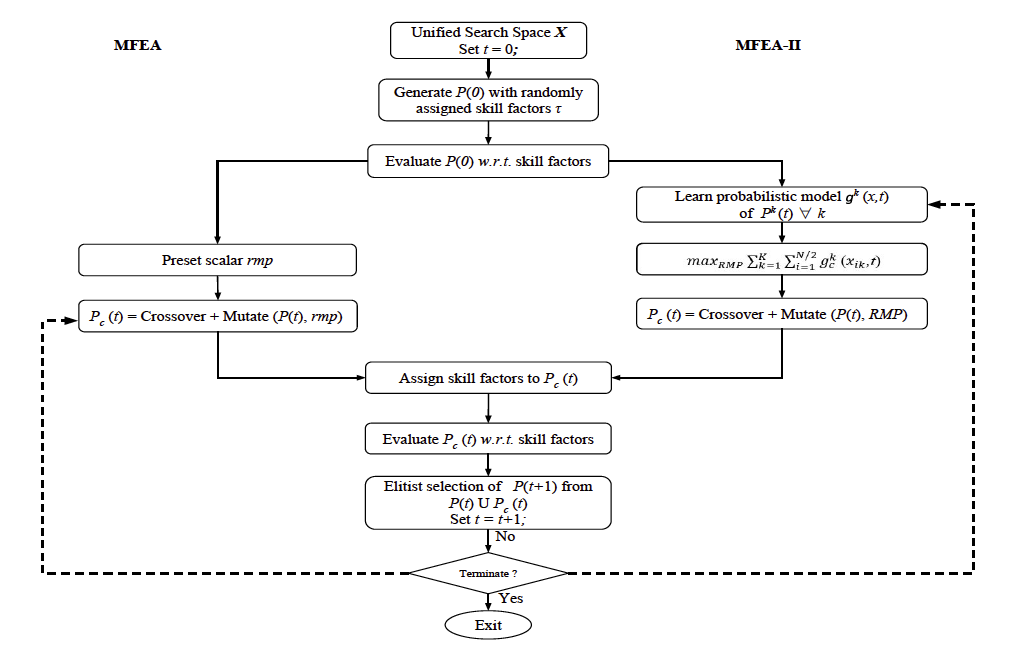
\includegraphics[width=15cm,height=12cm]{mfeaii.png}
        \caption{Lược đồ so sánh các bước thực hiện giải thuật MFEA-I và MFEA-II. Nguồn \cite{bali2019multifactorial}}.
        \label{fig:mfeaii}
    \end{figure}
    Hình \ref{fig:mfeaii} mô tả một góc nhìn tổng quan về sự khác biệt giữa MFEA và MFEA-II. Trong đó có thể chia 2 thuật toán này làm 3 pha chính theo thứ tự từ trên xuống: khởi tạo, trao đổi chéo, đánh giá và lựa chọn. Dễ thấy sự giống nhau nằm ở pha đầu tiên và cuối cùng. Điểm khác biệt của MFEA-II trong phá thứ 2 bởi quá trình học trực tuyến ma trận $RMP$ với phương pháp đã được trình bày ở mục \ref{sub:rmp-learning}. Mô tả quá trình học trực tuyến ma trận $RMP$ dưới dạng mã giả trong thuật toán \ref{alg:online-rmp-learning}
    \begin{algorithm}[ht]
        \caption{Học trực tuyến ma trận $RMP$}
        \begin{algorithmic}[1]
            \State Xây dựng một mô hình phân phối ước lượng $g^k(x,t)$ trên mỗi tập cá thể $P^k(t)$. $\forall k \in {1,2,...K}$
            \State Tối ưu hóa mô hình hỗn hợp $\max_{RMP}\sum_{k=1}^{K}\sum_{i=1}^{N/2}\log{g_c^k(x_{ik},t)}$
        \end{algorithmic}
        \label{alg:online-rmp-learning}
    \end{algorithm} \\
    Pha trao đổi khác tác vụ sẽ được mô tả trong thuật toán 5, khi các giải pháp được trao đổi giữa các tác vụ sẽ phụ thuộc vào ma trận $RMP$ đã học ở thuật toán \ref{alg:inter-task crossover}. Trong trường hợp ma trận $RMP$ học được toàn giá trị $0$ thì MFEA-II sẽ hoạt động tương tự với thuật toán tiến hóa kinh điển trong việc học song song từng tác vụ đơn lẻ. \\ 
    \begin{algorithm}[h!]
        \caption{Trao đổi khác tác vụ trong MFEA-II}
        \begin{algorithmic}[1]
            \State Chọn 2 cá thể ngẫu nhiên $x_i$ và $x_j$ từ quần thể $P(t)$:
            \If {$(\tau_i  \neq \tau_j)$}
                \If {$rand \leq rmp_{\tau_i,\tau_j}$}
                    \State $[x_a, x_b]$ $\leftarrow$ \emph{Trao đổi khác tác vụ} giữa $x_i$ và $x_j$;
                    \State Mỗi cá thể con cái sinh ra sẽ được gán ngẫu nhiên một giá trị thuộc tính kĩ năng $\tau_i$  hoặc $\tau_j$;
                \Else 
                    \State Lựa chọn ngẫu nhiên $x_i^{'}$ với thuộc tính kĩ năng $\tau_i$;
                    \State $[x_a]$ $\leftarrow$ \emph{Trao đổi cùng tác vụ} giữa $x_i$ và $x_i^{'}$;
                    \State Gán cá thể con cái $x_a$ với thuộc tính kĩ năng $\tau_i$;
                    \State Lựa chọn ngẫu nhiên $x_j^{'}$ với thuộc tính kĩ năng $\tau_j$;
                    \State $[x_b]$ $\leftarrow$ \emph{Trao đổi cùng tác vụ} giữa $x_i$ và $x_i^{'}$;
                    \State Gán cá thể con cái $x_b$ với thuộc tính kĩ năng $\tau_j$;
                
        \end{algorithmic}
        \label{alg:inter-task crossover}
    \end{algorithm}
     Tuy nhiên tại sao lại sử dụng MFEA-II để huấn luyện mạng neural trong khi các thuật toán huấn luyện mạng neural kinh điển sử dụng phương pháp gradient-based vẫn đang được hầu hết các nhóm nghiên cứu sử dụng. Trong chương tiếp theo, đồ án sẽ trình bày các yêu cầu cấp thiết của việc áp dụng này và qua đó là đề xuất, giải thuật áp dụng chi tiết.
    
\section{Tổng quan mạng neural}
    \subsection{Đơn vị nơ-ron cơ bản}
    Tương tự như thuật toán tiến hóa, mạng neural hay còn gọi là mạng neural nhân tạo thần kinh nhân tạo (thuật ngữ gốc: \emph{Artificial Neural Network - ANN}) \cite{hassoun1995fundamentals} cũng là một ý tưởng được lấy cảm hứng từ mạng các nơ-ron (thuật ngữ gốc: \emph{neuro}) thần kinh của con người. Trong đó, nơ-ron thần kinh là một đơn vị cơ bản cấu tạo hệ thống thần kinh quan trọng nhất của bộ não, nó có cấu trúc được mô tả như hình bên dưới:
    \begin{figure}[ht]
        \centering
        \scalebox{0.9}{\fbox{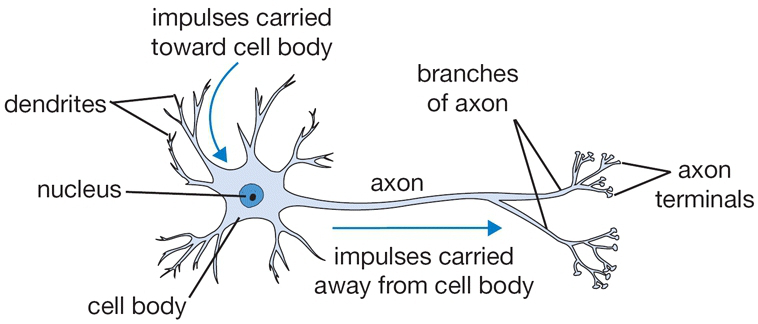
\includegraphics[width=\linewidth]{neuron-human.png}}}
        \caption{Cấu trúc của một perceptron đơn lẻ}
        \label{fig:problem:human-neuron}
    \end{figure}
    Một đơn vị nơ-ron đơn lẻ được gọi là \emph{perceptron} \cite{stephen1990perceptron}. Từ mô hình của perceptron được mô tả trong hình \ref{fig:problem:human-neuron} có thể thấy mỗi một nơ-ron sẽ nhận nhiều đầu vào nhưng chỉ cho ra một kết quả duy nhất. Được biểu diễn dưới dạng mô hình như sau:
    \begin{figure}[ht]
        \centering
        \fbox{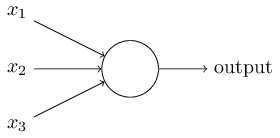
\includegraphics[width=0.7\linewidth]{perceptron.png}}
        \caption{Cấu trúc của một perceptron nhân tạo}
        \label{fig:problem:perceptron}
    \end{figure}
    Một perceptron sẽ nhận một hoặc nhiều đầu $x$ vào dạng nhị phân và cho ra một kết quả $o$ dạng nhị phân duy nhất. Các đầu vào được điều phối tầm ảnh hưởng bởi các tham số trọng lượng tương ứng $w$ của nó, còn kết quả đầu ra được quyết định dựa vào một ngưỡng quyết định $b$ nào đó.
    \subsection{Kiến trúc của ANN}
    ANN là kết hợp của các tầng perceptron hay còn gọi là perceptron đa tầng. 
    \begin{figure}[ht]
        \centering
        \scalebox{0.8}{\fbox{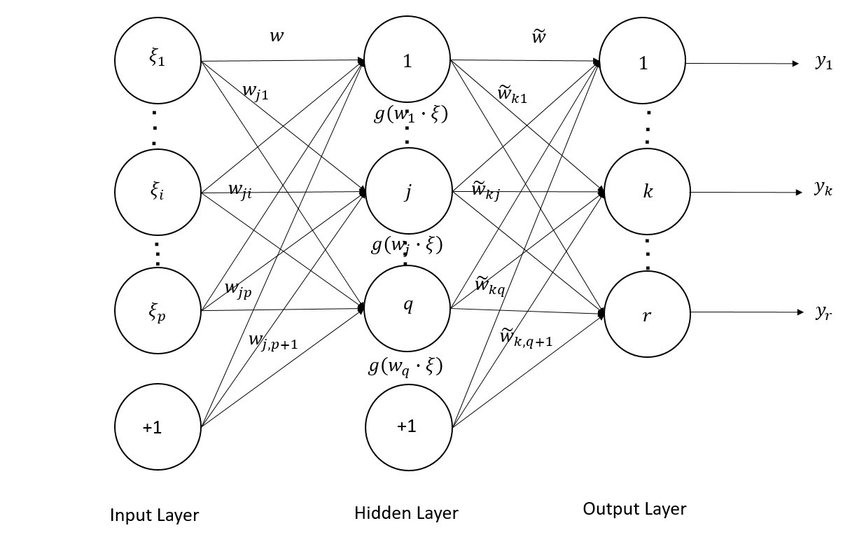
\includegraphics[width=\linewidth]{ff-neural.png}}}
        \caption{Kiến trúc ANN}
        \label{fig:problem:neural-architect}
    \end{figure}
    Một kiến trúc của ANN bao gồm 3 kiểu tầng chính:
    \begin{enumerate}
        \item \textbf{Tầng vào} (input layer): Là tầng bên trái cùng của mạng thể hiện cho đầu vào của mạng.
        \item \textbf{Tầng ẩn} (hidden layer): Là tầng nằm giữa tầng vào và tầng ra của mạng thể hiện cho các suy luận logic của mạng.
        \item \textbf{Tầng ra} (output layer): Là tầng nằm bên phải cùng của mạng thể hiện cho các đầu ra của mạng. Một mạng có thể có một hoặc nhiều đầu ra.
    \end{enumerate}
    Ở mỗi tầng, số lượng các nút mạng (nơ-ron) có thể khác nhau tuỳ thuộc vào bài toán và cách giải quyết. Nhưng thường khi làm việc các tầng ẩn thường có số lượng nơ-ron bằng nhau. 
    \subsection{Mạng neural lan truyền tiến}
    Như hình \ref{fig:problem:neural-architect} có thể thấy tất các nút mạng được kết hợp đôi một với nhau theo một chiều duy nhất từ tầng vào đến tầng ra. Tức là mỗi nốt ở tầng nào đó sẽ nhận đầu vào từ các nốt ở tầng trước đó mà không có chiều suy luận ngước lại. Hay nói cách khác ANN là này là một mạng lan truyền tiến \cite{fine2006feedforward}. 
    \begin{equation}
      \begin{array}{l}
        z_i^{l+1} = \sum_{j=1}^{n^{(l)}}w_{ij}^{(l+1)}a_j^{(l)} + b_j^{(l+1)} \\
        \\
        a_i^{(l+1)} = g(z_i^{(l+1)})
      \end{array}
    \end{equation}
    Trong đó $n^{(l)}$ là số lượng nút ở tầng $l$ tương ứng và $a_j^{(l)}$ là nút mạng thứ $j$ của tầng $l$. Còn $w_{ij}^{(l+1)}$ là tham số trọng lượng đầu vào $a_j^{(l)}$ đối với nút mạng thứ $i$ của tầng $l+1$ và $b_j^{(l+1)}$ là độ lệch thiên kiến (bias) của nút mạng thứ $i$ tầng thứ $l+1$. Đầu ra của nút mạng này được biểu diễn bằng $a_i^{(l+1)}$ ứng với hàm kích hoạt $g(z_i)$ tương ứng. Và riêng với tầng vào (input layer), thông thường $a^{(1}$ cũng chính là các đầu vào $x$ tương ứng của mạng. 
    \subsection{Huấn luyện mô hình mạng neural}
    Trong mục này chúng ta sẽ cùng bàn luận về một số các cách tiếp cận chính cho vấn đề huấn luyện mô hình ANN.
    Trước khi giải thích làm thế nào để huấn luyện một ANN thì ta sẽ cần định nghĩa về hàm lỗi (thuật ngữ gốc: \emph{loss function}). Hàm lỗi là hàm cho ta biết mạng hiện tại đang tốt như thế nào trên một tác vụ, bộ dữ liệu cụ thể. Một cách tiếp cận trực quan và đơn giản nhất mà ta có thể nghĩ ra đó là sử dụng hàm trung bình bình phương lỗi (thuật ngữ gốc: \emph{Min Square Error - MSE}).
    \begin{equation}
      L(y, \widehat{y}) = \frac{1}{m}\sum_{i=1}^m(y_i - \widehat{y_i})^2
    \end{equation}
    Với $\widehat{y}$ là giá trị ước lượng từ mạng, $y$ là giá trị thực tế từ bộ dữ liệu huấn luyện. Nếu giá trị hàm lỗi lớn chứng tỏ mô hình mạng nơ-ron của ta chênh lệch nhiều, chưa đưa ra kết quả tốt. Nhiệm vụ của ta sẽ là tối ưu bộ tham số $(w,b)$ sao cho hàm lỗi nhỏ nhất có thể. Và đây cũng là ý tưởng chính trong việc huấn luyện mô hình ANN. Để thực hiện nhiệm vụ tối ưu này, có 2 lớp phương pháp chính:
    \begin{itemize}
        \item Lớp thuật toán sử dụng phương pháp \textbf{gradient-based}.
        \item Lớp thuật toán \textbf{tiến hóa - EA}.
    \end{itemize}
    \subsubsection{Phương pháp Gradient Based}
    Hầu hết các nhóm nghiên cứu đều sử dụng phương pháp gradient-based để huấn luyện mạng nơ-ron hơn là sử dụng các phương pháp tiến hóa. Trong đó một phương pháp kinh điển, là nền tảng của các phương pháp khác đó là \emph{Grdient Descent - GD}.
    
    GD và các biến thể của nó là một trong những phương pháp phổ biến
    nhất. Ý tưởng chung là xuất phát từ một điểm mà chúng ta coi là gần với nghiệm
    của bài toán, sau đó dùng một phương pháp lặp để tiến dần đến điểm cần tìm,
    tức đến khi đạo hàm gần với 0 \cite{lecun2015deep}. 
    
    Giả sử ta tối ưu một hàm 1 biến $f(x), x\in \mathbb{R}$, gọi $x^*$ là tối ưu cục bộ của bài toán. Giả sử 1 điểm $x_t$ gần $x^*$, tại đó $f^'(x_t) > 0$ thì hướng tốt nhật để cập nhật $x_t$ là đi ngược hướng với đạo hàm tại đó. Trong GD, người ta cập nhật $x_{t+1}=x_t - \eta f^'(x_t)$, với $\eta$ được gọi là tốc độ học (thuật ngữ gốc: \emph{learning rate}). Hướng cập nhật tham số theo GD giúp nhanh chóng tối ưu đến một điểm cục bộ tương ứng với điểm xuất phát ban đầu. Đây là cách tiếp cận trục quan nhất và là công cụ chính để phát triển các thuật toán phức tạp hơn.
    \begin{figure}[ht]
        \centering
        \fbox{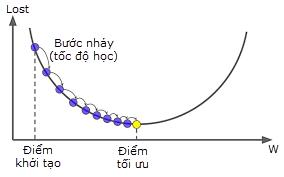
\includegraphics[width=0.4\linewidth]{gd.jpg}}
        \caption{Minh họa cách cập nhật tham số của gradient descent}
        \label{fig:gd}
    \end{figure}
    Từ nhận xét trên, người ta xây dựng công thức cập nhật cho hàm nhiều biến $f(\theta)$ ($\theta$ thường được dùng để ký hiệu tập tham số của mô hình cần tối ưu) như sau:
    \begin{equation}
        \theta_{t+1} = \theta_t - \eta \bigtriangledown_\theta f(\theta_t)
    \end{equation}
    Bắt ngưồn từ GD, rất nhiều các giải thuật dẫn xuất được phát triển dựa vào việc cải tiến về điểm khởi tạo, hoặc
    bước nhảy, có thể cố định hay di động, hoặc cải tiến hướng cập nhật tham số với đạo hàm có thêm các yếu tố giúp thuật toán vượt qua được các tối ưu cục bộ và tiến gần hơn đến tối ưu toàn cục. 
    \subsubsection{Vấn đề của phương pháp Gradient-Based}
    Ngoài ra còn rất nhiều các biến thể khác của SGD như Lan truyền ngược trung bình bình phương lỗi (thuật ngữ gốc: Root Mean Square Propagation - RMSProp) \cite{tieleman2012lecture}, Gia tốc cho đạo hàm Nesterov (thuật ngữ gốc: Nesterov Accelerated Gradient - NAG) \cite{nesterov2013gradient}, Adam \cite{kingma2014adam}... Các thuật toán này về cơ bản đều thực hiện rất nhanh và có những thành công trên những bộ dữ liệu nhất định ở nhiều lĩnh vực khác nhau. Tuy nhiên, chúng tồn tại những nhược
    điểm cố hữu của các phương pháp dựa trên đạo hàm:
    \begin{itemize}
        \item Với các bài toán học tăng cường, giá trị đầu ra thường là ước lượng nên việc áp dụng phương pháp sử dụng gradient-based gặp trở ngại lớn.
        \item Các mô hình ANN thực tế với rất nhiều tham số tạo nên một không gian tìm kiếm đa chiều phức tạp với rất nhiều điểm tối ưu cục bộ, điểm yên ngựa, bình nguyên (thuật ngữ gốc: plateau) hay các vùng phẳng \cite{eldan2016power, kawaguchi2016deep, miikkulainen2019evolving}. Những trở ngại đó khiến cho việc tìm ra tối ưu toàn cục là rất khó khăn, đòi hỏi khối lượng tính toán lớn và phải có sự tham gia của con người trong những thực nghiệm lặp đi lặp lại nhàm chán.
    \end{itemize}
    
    Để giải quyết các thách thức này đòi hỏi chúng ta cần đưa ra những hướng giải quyết mới có thể là thay đổi GD hoặc áp dụng những phương pháp tối ưu hóa khác có khả năng vượt trội, và thuật toán tiến hóa có thể là một ứng viên tiềm năng như vậy. EA đưa ra một chiến lược tự thích nghi với môi trường được xem như là một công cụ hữu hiệu để tối ưu trọng số kết nối mà không phải quan tâm đến việc tính đạo hàm \cite{whitley1990genetic}. Để tối ưu trọng sô, EA sẽ dùng chiến lược mã hóa nhị phân hoặc mã hóa số thực rồi coi việc học ANN là một bài toán tối ưu hóa liên tục \cite{yao1999evolutionary}. Nhờ vậy EANN có thể xử lý các trường hợp phức tạp, hàm không khả vi, đa cực trị hay có nhiều điểm yên ngựa... (vốn xảy ra càng nhiều khi ANN càng sâu và càng có nhiều tham số). Một số nhóm nghiên cứu nổi tiếng như Google Brain, OpenAI, Uber \cite{wong2018transfer, salimans2017evolution} đã đưa ra những nghiên cứu trong việc áp dụng giải thuật tiến hóa trong việc huấn luyện ANN để giải quyết bài toán. 
    Bởi vậy từ các mục tiếp theo trở đi, chúng ta sẽ đi vào tìm hiểu - phương pháp thứ 2 sử dụng ý tưởng tiến hóa để huấn luyện mạng neural. 
\section{Giới thiệu tiến hóa đa nhiệm trong huấn luyện mạng neural}
    \subsection{Cách tiếp cận tiến hóa trong huấn luyện mạng neural}
    \subsubsection{Định nghĩa}
    Phương pháp sử dụng thuật toán tiến hóa để huấn luyện mạng neural hay còn gọi là neuroevolution \cite{floreano2008neuroevolution} xem vấn đề cần học giống như một bài toán tối ưu hộp đen (thuật ngữ gốc: \emph{black-box optimisation}) nơi các giải pháp được cải thiện qua các thế hệ tiến hóa. Neuroevolution sử dụng thuật toán tiến hóa để xây dựng, huấn luyện ANN bao gồm các tham số, cấu trúc của mạng. Trong neuroevolution, một mẫu gen (thuật ngữ gốc: \emph{gennotype}) là kiểu cá thể của quần thể sẽ được ánh xạ với các tham số trong ANN. Qua mỗi thế hệ tiến hóa các cá thể sẽ được đánh giá dựa theo hàm đánh giá tương ứng với bài toán để chọn lọc và tiếp tục xây dựng thế hệ tiếp theo.
    \subsubsection{Các loại mã hóa}
    Một vấn đề cần quan tâm khi huấn luyện mạng neural bằng phương pháp tiến hóa đó là việc mã hóa từ mô hình mạng (ví dụ mô hình mạng trong hình \ref{fig:problem:neural-architect} về các cá thể như thế nào. Trong neuroevolution ta có 2 phương pháp mã hóa cá thể là:
    \begin{itemize}
        \item \textbf{Mã hóa trực tiếp} (thuật ngữ gốc: \emph{Direct-Encoding}: Là phương pháp mã hóa trực tiếp các thông số của mạng, giá trị các nơ-ron trong mạng vào những vị trí cụ thể trong kiểu gen.
        \item \textbf{Mã hóa gián tiếp} (thuật ngữ gốc: \emph{Indirect-Encoding}: Là phương pháp mã hóa gián tiếp theo cách tạo ra một mô hình mạng từ kiểu gen cụ thể.
    \end{itemize}
    Mỗi phương pháp mã hóa sẽ phụ thuộc vào kiểu bài toán mà nó giải quyết. 
    \subsection{Dạng bài toán áp dụng tiến hóa đa nhiệm trong huấn luyện mạng neural}
    Tuy nhiên một vấn đề nảy sinh trong việc huấn luyện ANN đó là việc không khai thác được những tri thức đã học được trong các mô hình đã học được trước đó. Chẳng hạn với bài toán huấn luyện mô hình học tăng cường, khi thông số môi trường thay đổi thì ta cần phải huấn luyện lại từ đầu mà không tận dụng được bất kỳ tri thức nào trước đó.
    Bằng ý tưởng của thuật toán tiến hóa đa nhiệm đã được trình bày ở phần trên thì việc áp dụng thuật toán vào huấn luyện nhiều ANN đồng thời có thể giải quyết được vấn đề này. Tiến hóa đa nhiệm sẽ khai phá được mối quan hệ tiềm ẩn giữa các tác vụ có liên quan đến nhau, qua đó đẩy nhanh tốc độ hội tụ của các tác vụ.
    
    Cần phải lưu ý rằng chữ \textit{tác vụ} khi áp dụng tiến hóa đa nhiệm vào huấn luyện ANN có thể hiểu theo nhiều nghĩa.
    \begin{itemize}
        \item \textbf{Bài toán thứ nhất}: Coi mỗi tác vụ là một bộ dữ liệu có số lượng hoặc tính chất của thuộc tính khác nhau.
        \item \textbf{Bài toán thứ hai}: Coi mỗi tác vụ tương ứng với một cấu trúc ANN khác nhau.
    \end{itemize}
    \begin{figure}[ht]
        \centering
        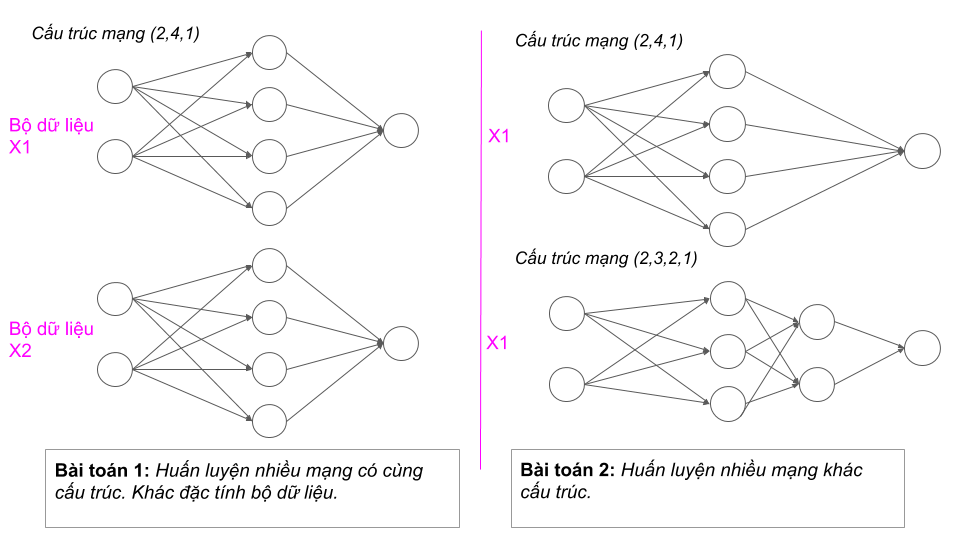
\includegraphics[width=1.0\linewidth]{images/neural-problem.png}
        \caption{Các loại bài toán huấn luyện tham số ANN}
        \label{fig:problem:neural-problem}
    \end{figure}
    Như trong hình \ref{fig:problem:neural-problem} mỗi định nghĩa về tác vụ sẽ tương ứng với một lớp bài toán khác nhau cần xây dựng mô hình riêng để giải quyết. Trong đồ án này tôi sẽ đưa ra các đề xuất của mình để giải quyết lần lượt cả 2 lớp bài toán trên.
    \begin{itemize}
        \item Với lớp bài toán thứ nhất tôi sẽ trình bày ở chương \ref{chap:problem_rl} trong việc áp dụng tiến hóa đa nhiệm trong việc huấn luyện mô hình học tăng cường trên nhiều môi trường đồng thời.
        \item Với lớp bài toán thứ hai tôi sẽ trình bày tại chương \ref{chap:problem} trong việc áp dụng tiến hóa đa nhiệm huấn luyện nhiều ANN với cấu trúc khác nhau.
    \end{itemize}
    Tương ứng với mỗi bài toán tôi sẽ đề xuất những giải thuật, chiến lược áp dụng tiến hóa đa nhiệm của mình. Đương nhiên mỗi vấn đề đều có những khó khăn, thách thức riêng, tuy nhiên qua quá trình giải những bài toán như vậy sẽ làm rõ hơn việc tư tưởng tiến hóa, đặc biệt là tiến hóa đa nhiệm có thực sự phù hợp trong huấn luyện ANN hay không.
    
    Lưu ý rằng tiến hóa đa nhiệm mà tôi nhắc tới sẽ là việc áp dụng đồng thời cả MFEA và MFEAII. Trong đó MFEA-II sẽ là thuật toán chủ yếu tôi muốn trình bày và MFEA sẽ là thuật toán cơ sở để so sánh, bên cạnh thuật toán tiến hóa thông thường.
    

